%% SectorQ paper: SIGMETRICS'27 (POMACS, acmsmall), the format of ScaleQsim (SIGMETRICS'26).
%% Build: module load texlive/2024; bash scripts/build.sh   (output in build/main.pdf)
%% Style check: python3 scripts/check_style.py               (0 findings before a draft is shown)
\documentclass[acmsmall,screen,nonacm,review]{acmart}

\usepackage{amsmath}
\usepackage{booktabs}
\usepackage{graphicx}
\usepackage{xcolor}
\usepackage{tikz}
\usepackage{caption}
\usepackage{subfig}
\usepackage{multirow}
\usepackage{makecell}
\usepackage{xspace}
\usepackage{comment}

\newcommand{\SectorQ}{\textit{SectorQ}\xspace}
\newcommand{\cuPP}{\textit{cuPauliProp}\xspace}
\newcommand{\todo}[1]{\textcolor{red}{[TODO: #1]}}
% placeholder for a figure that is not drawn for the paper yet: the source it will be redrawn from
\newcommand{\figsource}[1]{\fbox{\parbox{0.9\linewidth}{\centering\small\ttfamily #1}}}
% a data panel or legend strip of figures/make_paper_figures.py: drawn at 1/0.6 of its printed size, so every panel
% prints its text at one size (7.2 pt)
\newcommand{\panel}[1]{\includegraphics[scale=0.6]{figures/#1}}

\AtBeginDocument{\providecommand\BibTeX{{Bib\TeX}}}

\begin{document}

\title{SectorQ: Highly Scalable Pauli Propagation on HPC Systems with Window-Conserved Parity Sectors}

\author{Anonymous Author(s)}
\affiliation{\institution{Submission under review}\country{Anonymous}}

\begin{abstract}
% FORMAT: five sentences, 140-180 words (see the draft in 0.Abstract.tex)
% DRAFT (2026-10-14): five sentences, 140-180 words; numbers from README 1.5 (16 GPUs: as-is cuPauliProp; 512 GPUs: reach)
This paper presents \SectorQ, a Pauli propagation system designed to compute the expectation values of quantum circuits with more than 100 qubits on GPU clusters.
As tighter coefficient cutoffs increase the number of kept terms, the terms of a 127-qubit circuit exceed the memory of hundreds of GPUs, and the existing multi-GPU engine merges them across all GPUs after every gate.
\SectorQ introduces window-conserved parity sectors, which divide the terms by the parities that every gate of a window leaves unchanged and keep each new term in the same sector as its merge partner.
With this design, \SectorQ applies each window without exchanging terms between nodes, balances the sectors by choosing the parities at run time from a sample of the live terms, and holds the sectors in host memory beyond the capacity of the GPU memory.
Our evaluation using seven circuits on up to 512 NVIDIA A100 GPUs shows that \SectorQ reduces the simulation time of \cuPP on 16 GPUs by 4.4-9.7$\times$ and increases the largest finished problem on 512 GPUs by 140$\times$.

\end{abstract}

\maketitle

\section{Introduction}
\label{sec:intro}
% ScaleQsim order: context, need, representations, constraints, prior work, design, contributions.

Quantum processors with more than 100 qubits have enabled experiments beyond sampling demonstrations, including measurements of observables in interacting physical models~\cite{arute2019quantum,kim2023evidence}.
Observable expectation values characterize quantities such as magnetization and energy in quantum simulation, with applications in physics, chemistry, and materials science~\cite{georgescu2014simulation}.
For example, a 127-qubit processor measured the magnetization of a kicked Ising model at a scale beyond direct state-vector simulation~\cite{kim2023evidence}.
Classical calculations of these observables provide a basis for assessing the accuracy and computational cost of the quantum experiment.
The tractable circuit size depends on the classical representation, its approximation, and the computing resources available for the calculation.

Current processors remain noisy intermediate-scale quantum (NISQ) devices, with errors that affect measured expectation values~\cite{preskill2018quantum}.
Error mitigation estimates an observable from repeated measurements, including measurements at amplified noise levels~\cite{kim2023evidence}.
Classical simulation on high-performance computing (HPC) systems provides an independent reference for evaluating these estimates.
Such references support hardware validation, error-mitigation assessment, and algorithm development, subject to the numerical error of the classical method.
Tensor network and Pauli propagation studies have reproduced observables from the 127-qubit experiment~\cite{tindall2024efficient,begusic2024fast}.
These calculations establish the relevance of classical simulation even when a full state vector exceeds available memory.

Three representations are relevant to the classical simulation of these circuits.
State vector simulation stores all $2^n$ complex amplitudes of an $n$-qubit state, requiring 16~PiB for 50 qubits in double precision~\cite{haner2017petabyte}.
Tensor network simulation represents the state through tensors, with contraction cost determined by the network structure and the required tensor dimensions~\cite{tindall2024efficient}.
Pauli propagation represents an observable as a sum of Pauli strings and propagates it through the circuit in the Heisenberg picture~\cite{begusic2024fast,rudolph2025pauli}.
Its storage and execution costs depend on the number of retained terms as well as the string length and gate sequence.
Current NVIDIA and IBM libraries support this representation~\cite{cupauliprop,qiskitpauliprop}.
Our work focuses on distributed Pauli propagation, where coefficient truncation controls the retained expansion and permits calculations beyond the memory range of full state vectors.

The retained expansion can exceed the capacity of one GPU as the coefficient cutoff decreases.
Terms also accumulate between scheduled truncations, requiring temporary storage beyond the retained expansion.
For the 127-qubit kicked Ising circuit, the maximum population at a window boundary increases from 159 million terms at cutoff $10^{-5}$ to 11.9 billion at $10^{-6}$.
At 40 bytes per term, these populations require about 6.4~GB and 475~GB before execution buffers.
Distributed implementations address this storage requirement on GPU clusters and on CPU systems, including Fugaku runs with $2^{17}$ processes~\cite{cupauliprop,orqa}.
However, the distributed GPU implementations still incur coordination costs at individual gates and require their local expansions to fit device memory.

%   시스템별 나열을 빼고 원인 두 가지(gate마다의 전역 단계, GPU 메모리)와 메모리가 모자라는 이유를 씀. 시스템별 배수는 평가로.
Distributed GPU propagation has two principal constraints.
First, terms with the same Pauli string must be merged before coefficient truncation, including contributions produced on different GPUs.
The distributed mode of \cuPP coordinates this merge after every gate~\cite{cupauliprop}.
The measured fixed cost increases from 5.9~ms per gate on four GPUs to 29.8~ms on 16 GPUs.
Second, device memory must accommodate retained terms, intermediate branches, and merge workspace.
An anticommuting rotation can produce two terms from one input, increasing the expansion between truncations.
Under these requirements, \cuPP retains about 100 million terms per GPU with a 36~GB memory budget.
The GPU implementation of paulistrings-rs also stores its assigned partitions in device memory~\cite{paulistrings}.
Deferred deduplication reduces global merge frequency but increases storage for duplicate strings.
Thus, a distributed design must provide merge locality across multiple gates and accommodate the stored operator beyond the working buffers of individual GPUs.

\begin{table}[t]
\caption{Features of Pauli propagation systems}
\label{tab:prior}
\centering
\small
\begin{tabular}{@{}llccccc@{}}
\toprule
\textbf{System} & \textbf{Method} & \textbf{MN} & \textbf{GPU} & \textbf{LP} & \textbf{RP} & \textbf{HM} \\
\midrule
PauliPropagation.jl~\cite{rudolph2025pauli} & Pauli propagation, one node & & & & & \\
SPD~\cite{spd} & Sparse Pauli dynamics & & \checkmark & & & \\
ORQA~\cite{orqa} & Structured distribution map & \checkmark & & & & \\
MonoProp~\cite{monoprop} & Distributed Pauli propagation & \checkmark & & & & \\
\cuPP~\cite{cupauliprop} & Global merge after every gate & \checkmark & \checkmark & & & \\
paulistrings-rs~\cite{paulistrings} & Fixed linear partition & \checkmark & \checkmark & \checkmark & & \\
\midrule
\textbf{\SectorQ (Ours)} & \textbf{Window-conserved parity sectors} & \checkmark & \checkmark & \checkmark & \checkmark & \checkmark \\
\bottomrule
\end{tabular}
\par\smallskip
\begin{minipage}{\linewidth}\footnotesize
MN denotes multi-node execution, GPU device execution, LP locality-preserving partitions, RP run-time partitions derived from gates and live terms, and HM host storage beyond GPU capacity.
\end{minipage}
\end{table}

Previous systems address arithmetic, distribution, and storage at different levels, as summarized in Table~\ref{tab:prior}.
Single-node simulators use sparse data structures, circuit symmetries, and GPU kernels to reduce propagation cost~\cite{begusic2024fast,rudolph2025pauli,spd}.
ORQA uses a structured distribution map to limit communication partners, and MonoProp supports distributed CPU propagation~\cite{orqa,monoprop}.
The distributed mode of \cuPP combines contributions across GPUs after individual gates~\cite{cupauliprop}.
The linear partition in paulistrings-rs assigns strings through fixed bit parities, with a predictable communication partner when a generator changes a partition label~\cite{paulistrings}.
Commutator-graph analysis also identifies operator subspaces invariant under a set of generators~\cite{west2025graph}.
None of these implementations combines window-conserved rows, row selection from live terms, and host-memory sector execution.

\SectorQ constructs a partition for each window of consecutive gates and selects its rows during execution.
The window generators define conserved parities that assign every contribution to an equal Pauli string to the same sector.
The runtime selects among these parities using a sample of the live terms, then assigns each sector to one node for the window.
This assignment confines merge and truncation to sector execution until the next window boundary.
The host-memory store retains the sectors, and each GPU loads one sector at a time with the workspace required by the propagation library.
An oversized sector is subdivided using further rows valid for its remaining operations.
Operator capacity consequently depends on distributed host storage and the availability of executable sector subdivisions, while term exchange occurs at window boundaries.

% ¶8 "In this paper": ACCEPTED by the user (2026-10-14), keep as it is.
% (ScaleQsim형 대안 "The goal of SectorQ is to 1) 2) 3). To achieve these goals, SectorQ 1) 2) 3)."은 사용자가 고르면 바꿈)
In this paper, we present \SectorQ, a Pauli propagation system for GPU clusters that partitions the terms by the parities that a window of gates conserves.
A rotation gate maps each term to itself and to its product with the generator of the gate, and every parity that the generator leaves unchanged assigns the same value to both terms.
Specifically, \SectorQ introduces 1) window-conserved parity sectors that the system recomputes for every window from the generators of its gates, 2) a run-time choice of the parities and the number of sectors from a sample of the live terms while the GPUs process the current window, and 3) a host-memory sector store from which each GPU loads one sector at a time.
With these sectors, the terms move between nodes only at window boundaries, and the number of terms that \SectorQ holds follows the host memory of all nodes.
Our evaluation on up to 512 NVIDIA A100 GPUs of the Perlmutter supercomputer shows that \SectorQ reduces the simulation time by 4.4-9.7$\times$ on 16 GPUs and increases the largest finished problem by 140$\times$ on 512 GPUs compared with \cuPP, the existing multi-GPU engine.
We open-source \SectorQ at: \url{https://anonymous.4open.science/r/SectorQ}

\section{Background}
\label{sec:background}
% 구성(2026-10-14 사용자: "2.1과 2.2를 합치고, cascade처럼 실험 데이터로 필요성을" -> "섹션 3개로"):
%   2.1 Pauli propagation과 병목 둘(개념 + 정확도 데이터)  2.2 기존 분산 방식의 도전 둘(cuPauliProp 측정)
%   2.3 기회: 구간이 보존하는 parity, 고정 분할의 통신, 실행 중 분할 선택 -> 설계 메커니즘
% 근거: pauliprop/README.md 1.1, 2.2-2.4, 3.3, 4.4절; analysis/fixed_rows.py(회로 일곱 개의 구조, frame 없는 좌표),
%       analysis/geometric_rows.py(kicked Ising 덤프 둘), 엔진 로그의 windows= 줄; paulistrings-rs ARCHITECTURE.md 236행, docs 16행.
% 범위: "고정 분할은 gate마다 항을 옮긴다"는 frame 없이 gate를 항에 적용하는 기존 구현에 대한 말.
%       frame 위에서 첫 구간의 행을 고정하면 40-180개 연산에서만 옮김(analysis/fixed_rows.py) -> 평가의 고정 행 대 구간 행 비교가 답할 것.

\subsection{Pauli Propagation beyond 100 Qubits}
Pauli propagation represents an observable as a sparse sum of Pauli strings and applies circuit operations in the Heisenberg picture~\cite{begusic2024fast,rudolph2025pauli}.
The propagated observable is evaluated against the initial state to obtain an expectation value.
This representation has supported circuits with more than 100 qubits, with execution cost determined by the retained expansion, string length, and gate sequence.

\noindent\textbf{Branch, Merge, and Truncate.}
Each term consists of a coefficient and a Pauli string, represented by one x bit and one z bit per qubit.
The product of two strings corresponds to the XOR of their bit vectors, with the multiplication phase included in the coefficient.
A rotation with generator $Q$ preserves a commuting string and branches an anticommuting string $P$ into strings $P$ and $P\oplus Q$ with cosine and sine factors, respectively.
One rotation can consequently double the term population before merging.
The merge sums coefficients with identical strings, and truncation removes terms whose merged coefficient magnitude is below the cutoff.
Clifford operations map each string to one string, while the Pauli noise channels considered here scale coefficients without changing their strings (Figure~\ref{fig:pp}).
The expansion size changes at branching, merging, and truncation, requiring storage for intermediate terms as well as retained terms.

\noindent\textbf{Term Growth with the Coefficient Cutoff.}
The coefficient cutoff controls the retained expansion and affects the approximation error.
On a 30-qubit circuit with an exact reference, the absolute error is 0.019 at cutoff $10^{-3}$ and 0.00007 at $10^{-7}$.
On the 127-qubit kicked Ising circuit, the expectation value is 0.153 at cutoff $10^{-4}$, 0.229 at $10^{-5}$, and 0.322 at $10^{-6}$.
The largest boundary count rises to 159 million terms at cutoff $10^{-5}$ and 11.9 billion at $10^{-6}$.
The latter occupies about 475~GB at 40 bytes per term before execution buffers.
Within a window, we also sum the maximum term count reached by each sector execution.
The largest of these sums reaches 1.4 billion and 100 billion at the two cutoffs, respectively.
These sums quantify intermediate expansion across sector executions, whose maxima can occur at different times.
The boundary population measures stored operator size, while the sector maxima characterize the additional working-buffer requirement.

\noindent\textbf{Merge before Truncation.}
Coefficient truncation applies to the sum of all contributions with the same Pauli string.
Contributions from different input terms can individually fall below the cutoff even when their sum exceeds it.
Independent truncation of those contributions changes the retained operator.
For example, the 127-qubit kicked Ising circuit at cutoff $10^{-4}$ produces expectation values of 0.194-0.283 with truncation before the global merge, compared with 0.1531 after the merge.
The gate generator determines which input strings can contribute to an identical output string.
A distribution based only on the current locations of input terms cannot guarantee that these contributions are local.
A locality-preserving partition must constrain generator-induced changes to string labels while accommodating the expansion's storage requirements (Table~\ref{tab:sv_pp}).

\begin{table}[t]
\caption{Distribution of state vector simulation and Pauli propagation}
\label{tab:sv_pp}
\centering
\small
\begin{tabular}{@{}lll@{}}
\toprule
 & \textbf{State Vector} & \textbf{Pauli Propagation} \\
\midrule
Representation & $2^n$ amplitudes & Variable number of Pauli terms \\
Index space & Fixed amplitude indices & Strings retained during propagation \\
Gate operation & Updates indexed amplitudes & Branches, merges, and truncates terms \\
Remote dependence & Distributed amplitude indices & Equal strings across partitions \\
Storage requirement & $2^n$ complex amplitudes & Retained terms and intermediate expansion \\
\bottomrule
\end{tabular}
\end{table}

\begin{figure}[t]
\centering
\subfloat[Operations of one gate]{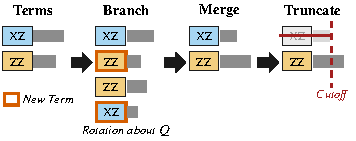
\includegraphics[scale=0.95]{figures/ops.pdf}}\hfill
\subfloat[Kicked Ising value]{\panel{bg_accuracy_a}}\hfill
\subfloat[30-qubit TFIM error]{\panel{bg_accuracy_b}}
\caption{Operations and accuracy of Pauli propagation}
\label{fig:pp}
\end{figure}

\subsection{Challenges in Distributed Pauli Propagation}
Distributed propagation must combine contributions across partitions before truncation and provide sufficient memory for intermediate expansion.
We examine these requirements in \cuPP~v0.5.0 using the 127-qubit kicked Ising circuit on NVIDIA A100 GPUs.

\noindent\textbf{Global Step after Every Gate.}
\cuPP performs a distributed merge after every gate because contributions to an identical string may reside on different GPUs.
Each MPI rank applies the gate to its local terms and issues 22 allgather calls during merge and redistribution in the measured trace.
These collectives occur even though 57\% of the gates exchange no terms.
This global step adds a fixed cost of 5.9, 22.5, and 29.8~ms per gate on 4, 8, and 16 GPUs, against 0.05-0.8~ms on one GPU (Figure~\ref{fig:anatomy}).
The measured workload reaches 22.5 million intermediate terms and takes 2.9-3.2~s on one GPU, compared with 33-48, 65, and 71~s on 4, 8, and 16 GPUs.
GPU computation occupies 9\% of execution time in this trace.
The largest rank holds 1.001 times the mean term count, indicating nearly uniform term distribution.
The increasing gate-level coordination cost limits performance despite this balance.

\noindent\textbf{Capacity Bound by the GPU Memory.}
\cuPP stores each rank's expansion and execution workspace in GPU memory.
Across the seven circuits, intermediate term counts reach 2.9-36 times the population at the start of a gate group.
Merge workspace requires additional memory alongside these intermediate terms.
\cuPP exhausts memory at 88-104 million retained terms per rank on 1-16 GPUs, although the retained payload occupies only about 4~GB of the 36~GB device-memory budget.
Deferred deduplication reduces merge frequency, but duplicate strings exhaust the memory of 16 GPUs in two of the seven circuits.
Without the global merge, local truncation also changes the expectation value to 0.1675 on four GPUs and 0.189 on 16 GPUs, compared with the merged value of 0.1531.
Available storage must accommodate intermediate expansion and workspace while preserving the merge required for coefficient truncation.

\begin{figure}[t]
\centering
\subfloat[Run time]{\panel{bg_time_a}}\hfill
\subfloat[Fixed cost per gate]{\panel{bg_gatecost_a}}\hfill
\subfloat[Terms per GPU at failure]{\panel{bg_capacity_a}}
\caption{Distributed mode of \cuPP}
\label{fig:anatomy}
\end{figure}

\subsection{Opportunity in Parities Conserved by Windows}
A partition conserved across several gates can permit local merge and truncation throughout those gates.
We examine the available conserved parities in seven circuits and their distribution over kicked Ising terms.

\noindent\textbf{Parities Conserved by Windows of Gates.}
A rotation with generator $Q$ can produce the string $P\oplus Q$ from $P$.
Every row $r$ satisfying $r\cdot Q=0$ assigns the same parity to both strings.
A window of consecutive gates conserves rows orthogonal to all its generators, permitting independent propagation within the resulting sectors.
Table~\ref{tab:windows} counts windows under a rule that retains at least $n$ independent conserved rows for an $n$-qubit circuit.
The seven circuits contain 1,100-7,960 gates and form 8-45 windows, reducing potential term-exchange boundaries by factors of 89-398 relative to gate boundaries.
The full circuits conserve at most two independent parities in this analysis, and their live terms have identical values on those parities.
Full-circuit conserved rows consequently cannot divide the measured expansions, whereas window-specific rows provide nontrivial partitions.

\noindent\textbf{Communication with Fixed Partitions.}
The linear partition in paulistrings-rs retains fixed rows throughout propagation~\cite{paulistrings}.
In the following analysis, gates act directly on strings without a Clifford frame.
A generator that changes a partition label requires inter-partition communication when the affected terms are present.
With 16 parts, random rows over all bits permit label changes at 93-96\% of the gates in the seven circuits, compared with 31-95\% for rows restricted to x bits or z bits.
On the kicked Ising circuit, random rows change the owner of 94\% of the terms at a layer of two-qubit gates, and rows over lattice regions reduce this share to 68-89\% with the largest of 16 parts at 1.65-3.37 times the mean.
The implementation lists automatic row selection as an open problem~\cite{paulistrings}.
A row change requires repartitioning the retained strings, making both its frequency and the resulting load balance relevant to execution cost.

\begin{table}[t]
\caption{Window counts and fixed-partition communication in seven circuits}
\label{tab:windows}
\centering
\small
\begin{tabular}{@{}lrrrrr@{}}
\toprule
\textbf{Circuit} & \textbf{Gates} & \textbf{Windows} & \makecell[r]{\textbf{Gates per}\\\textbf{Window}} & \makecell[r]{\textbf{Moving Gates}\\\textbf{(Random Rows)}} & \makecell[r]{\textbf{Moving Gates}\\\textbf{(z Rows)}} \\
\midrule
Kicked Ising & 5,420 & 20 & 271 & 94\% & 50\% \\
TFIM heavy-hex & 5,420 & 45 & 120 & 93\% & 50\% \\
Noisy kicked Ising & 7,960 & 20 & 398 & 95\% & 50\% \\
TFIM 11$\times$11 & 3,410 & 24 & 142 & 94\% & 60\% \\
XXZ 8$\times$8 & 2,048 & 23 & 89 & 94\% & 62\% \\
QAOA & 1,100 & 8 & 138 & 94\% & 60\% \\
Ansatz & 4,784 & 34 & 141 & 96\% & 95\% \\
\bottomrule
\end{tabular}
\end{table}

\noindent\textbf{Partition Selection from Live Terms.}
Window generators determine valid rows, while the distribution of live strings determines the population of each sector.
For kicked Ising at cutoff $10^{-5}$, the population at window starts increases from one to 159 million terms (Figure~\ref{fig:windows}).
Early windows have insufficient terms to occupy all GPUs, whereas later windows require multiple sectors per node.
Intermediate growth further changes sector sizes within a window.
A row set that balances one boundary population need not balance the population at another boundary, even when it remains algebraically valid.
The system can use the live distribution to select rows and sector counts subject to the conservation constraints.
This separation between validity and load balance permits a partition that preserves merge locality while adapting execution granularity to the retained operator.

\begin{figure}[t]
\centering
\panel{bg_windows_legend}\\[-2pt]
\subfloat[Gates and windows]{\panel{bg_windows_a}}\hfill
\subfloat[Terms at window starts]{\panel{bg_window_terms_a}}
\caption{Windows of gates in seven circuits}
\label{fig:windows}
\end{figure}

The design in Section~\ref{sec:design} combines window-conserved partitions with run-time row selection and host-memory sector storage.
The partition supplies merge locality, while host storage accommodates sectors beyond the working set of an individual GPU.

\section{SectorQ Design}
\label{sec:design}
\SectorQ addresses the locality and capacity limits with three mechanisms.
Window-conserved parity sectors assign equal-string contributions to the same sector throughout a group of gates.
Runtime re-sectoring selects the next partition from window generators and sampled live terms during execution.
Host-memory sector execution separates the stored expansion from the working set of each GPU and redistributes terms at window boundaries.

\subsection{Overall Architecture}
Figure~\ref{fig:overview} shows the circuit processing and the execution loop on each node.
The CPU constructs windows and selects their rows, host memory holds the sectors, and each GPU processes one sector at a time.

\noindent\textbf{Window Formation.}
The \emph{Window Builder} first expresses the circuit in the processing order of the observable.
A Clifford frame absorbs eligible Clifford gates and transforms the generators of subsequent rotations, preserving the action on the observable.
For example, a Hadamard maps the generator $Z_3$ to $X_3$ in the illustrated circuit.
For each window, the builder accumulates the span of the branching generators over $\mathrm{GF}(2)$ and stops before its dimension exceeds the number of qubits.
This bound ensures at least as many independent conserved rows as qubits for run-time partition selection.
The default boundary moves to the last scheduled truncation in the second half of the window when one is available, reducing the terms that require redistribution.
Clifford operations that remain explicit transform generators into a common coordinate system for this calculation.
The resulting window defines a sequence of operations and a space of valid partitions, with the particular rows selected during execution.

\noindent\textbf{Window Loop.}
Each node follows the numbered steps in Figure~\ref{fig:overview}.
At step (1), a GPU worker loads one sector from the \emph{Sector Store} in host memory.
At step (2), its \emph{Sector Executor} applies the current window, including the merges and scheduled truncations.
During these operations, \emph{Runtime Re-Sectoring} uses the CPU to select the rows of the next window.
At step (3), the worker uses these rows to partition its output on the GPU.
Step (4) appends output chunks to the host lists of the next sectors.
The \emph{Sector Exchanger} transfers the remote lists at step (5), assigning sector $d$ to node $d\bmod N$ among $N$ nodes.
Each node then processes its received sectors with the same loop.
The last window evaluates the observable against the input state and reduces the partial answers across nodes.
Each sector is complete before its next window begins, permitting the window's merges and truncations to execute locally.

\begin{figure}[t]
\centering
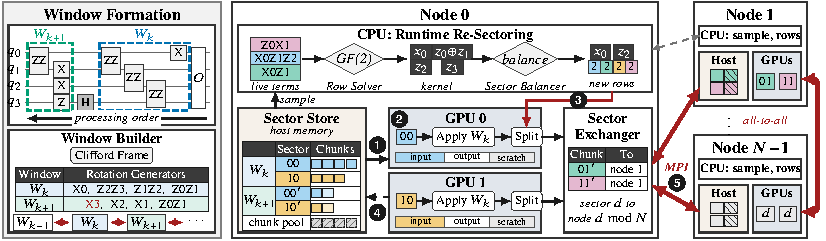
\includegraphics[width=\textwidth]{figures/overview.pdf}
\caption{Overall architecture of \SectorQ}
\label{fig:overview}
\end{figure}

\subsection{Window-Conserved Parity Sectors}
The execution loop requires a partition that preserves merge locality through every operation of a window.
Figure~\ref{fig:sectors} illustrates this condition on four qubits and two parity rows.

\noindent\textbf{Rows Conserved by a Window.}
A Pauli string has a binary representation $v=(x,z)\in\mathrm{GF}(2)^{2n}$, with its phase represented in the coefficient.
For a row $r$, the parity is the binary inner product $r\cdot v$.
A rotation with generator $q$ branches an anticommuting input string $v$ into $v$ and $v\oplus q$.
Their parities agree whenever $r\cdot q=0$.
The \emph{Row Solver} computes the annihilator of the generator span with Gaussian elimination over $\mathrm{GF}(2)$.
If that span has dimension $d$, its annihilator has dimension $2n-d$, at least $n$ under the window rule.
The selected rows form a matrix $R$, and the bit vector $Rv$ labels the sector of $v$.
This binary linear algebra is related to symmetry detection for qubit tapering~\cite{bravyi2017tapering}.
The rows label terms of the observable during one window, retaining the full qubit representation for subsequent windows.

\noindent\textbf{Merge Locality.}
Every descendant of a term retains its sector label through the branching rotations of the window.
This property follows by induction from $R(v\oplus q)=Rv$ for each generator in the window.
A coefficient change from a Pauli noise channel also preserves the string and its label.
For an explicit Clifford operation, the row coordinates transform with the strings to preserve the same label.
Equal strings have equal labels, placing all contributions to a string in one sector before truncation.
Consequently, a merge and coefficient truncation within each complete sector produce the same operator as a global merge and truncation at the same operations, apart from floating-point summation order.
In the example, the rows $x_1$ and $z_0\oplus z_1\oplus z_2\oplus z_3$ label both $Z_0X_1$ and $Y_0X_1$ as sector $11$.
The descendants retain label $11$ throughout $W_k$, allowing their coefficients to be combined before the scheduled truncation.

\noindent\textbf{Exchange Only at Window Boundaries.}
The next window can contain generators that change the current parity labels.
For example, $X_1$ in $W_{k+1}$ changes the parity $x_1$ used by $W_k$.
The runtime computes a new matrix for $W_{k+1}$ and regroups the output of $W_k$ before that window begins.
This regrouping collects all fragments of each next sector on its owner for merging before the next truncation.
The construction differs from a fixed linear partition~\cite{paulistrings}, whose rows can require a remote transfer at a gate that changes a partition label.
It also differs from a partition based only on symmetries of the full circuit, since these symmetries need not distinguish the live terms.
The window rule requires conservation only over the operations assigned to the current sector execution.
The resulting partitions can change at window boundaries while preserving the prescribed truncation schedule.

\begin{figure}[t]
\centering
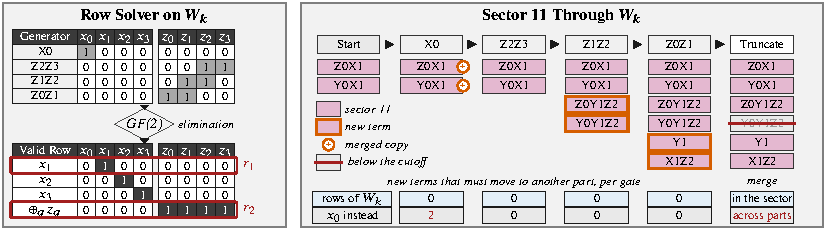
\includegraphics[width=\textwidth]{figures/sectors.pdf}
\caption{Window-conserved parity sectors}
\label{fig:sectors}
\end{figure}

\subsection{Runtime Re-Sectoring}
Conservation determines which rows are valid, but the live terms determine their load balance.
Figure~\ref{fig:resector} shows how the runtime selects the next rows while the GPUs process the current window.

\noindent\textbf{Sampling the Live Terms.}
At the start of a window, each node samples strings from its host sectors with a regular stride determined by the global term count.
The configured sample target is 200,000 terms across all nodes.
The CPU applies the current window's bit-changing Clifford operations to these strings before the next partition is scored.
This estimate applies coordinate changes without reproducing the branching and truncation of the sampled operator.
The sample approximates the string coordinates at the next boundary, with no exact prediction of the output population.
An MPI gather collects the samples on rank zero, where the row solver and the \emph{Sector Balancer} make a common decision for every node.
A broadcast distributes the selected rows and window description.
All workers use the broadcast matrix to assign identical labels to identical strings.
The sample affects performance decisions only, since every selected row must satisfy the generator constraints independently of the sampled terms.

\noindent\textbf{Balanced Row Selection.}
The sector balancer generates eight candidate row sets from random combinations of the annihilator basis.
For each candidate, it counts sampled strings per sector and selects the row set that minimizes the maximum count.
The illustrated pairs produce largest counts of eight, four, and two, and the selected pair $(x_0,z_2)$ divides the eight strings equally.
The number of rows depends on the estimated output size, the target terms per sector, and the available GPUs.
The estimate uses the previous window's observed growth with a bounded growth factor.
The runtime requests one task per GPU, or two when the preceding window exceeds the configured duration threshold, provided the resulting sectors remain sufficiently large.
Windows with few terms use fewer sectors to avoid small GPU tasks.
A configurable cap bounds the number of sectors at a boundary.
Candidate scoring controls the sampled maximum sector size, while the row count controls execution granularity and the number of available tasks.

\noindent\textbf{Overlap with the Running Window.}
The host sample is captured before the workers consume their input sectors.
After the workers start, the CPU main thread gathers the sample, computes the next window, scores the candidate rows, and broadcasts the result.
Workers need those rows only when they partition their output for the next window.
A worker that reaches this point before the rows are ready waits on a local condition variable.
The implementation records this wait separately from CPU selection time to distinguish overlapped selection from a delay visible to workers.
The overlap depends on the relative durations of row selection and sector execution.
Short windows can expose selection latency, whereas longer windows provide more time for the CPU calculation before output partitioning.
The conservation constraints ensure merge locality in both cases, independent of sample quality and the duration of selection.

\begin{figure}[t]
\centering
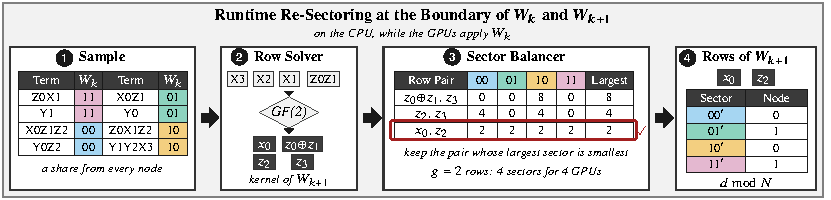
\includegraphics[width=\textwidth]{figures/resector.pdf}
\caption{Runtime re-sectoring at a window boundary}
\label{fig:resector}
\end{figure}

\subsection{Host-Memory Sector Execution and Exchange}
The selected sectors are units of execution rather than permanent GPU allocations.
Figure~\ref{fig:execution} shows their storage, processing, and transfer across a window boundary.

\noindent\textbf{Chunked Sector Store.}
The sector store represents each sector as a list of fixed-capacity host chunks, with 262,144 terms per chunk by default.
Each term contains a binary string and a double-precision coefficient.
A pool retains pinned chunks for reuse after GPU transfers or MPI sends, avoiding repeated registration for every sector.
The same chunk representation supports input loading, output collection, and reception from another node.
A sector can contain multiple chunks, and a node can hold more sectors than it has GPUs.
The live expansion occupies host memory, while only the sectors under execution require GPU buffers.
The total capacity depends on host storage for input, temporary output, and exchanged chunks.
Within a node, workers obtain sectors from a shared queue, initially ordered by decreasing size.
Workers obtain another sector as they finish their current task, redistributing work within the node as sector execution times vary.

\noindent\textbf{Sector Execution on GPUs.}
Each worker maintains input and output expansions together with the library workspace on its GPU.
The worker loads a complete sector, applies its window, and performs the required merges before coefficient truncation.
If the sector is too large to load with sufficient workspace, an additional valid row divides it in host memory.
If growth exhausts the GPU buffers during execution, the worker partitions the current expansion using a further row conserved by the remaining operations.
The resulting subsectors return to the local queue with the operation position and any pending merge or truncation.
Each subsector resumes from that position and preserves merge locality under the finer partition.
A split succeeds only if the available rows distinguish enough terms to fit the working set.
The runtime records host and GPU splits separately.
Host storage can accommodate a larger operator only when its sectors admit subdivisions whose expansions and workspace fit an individual GPU.

\noindent\textbf{Boundary Exchange.}
At the end of a window, a GPU partitions its surviving terms by the next matrix and copies them into host chunks.
Chunks for local sectors remain on the node, and the sector exchanger sends the other chunks to their owners.
The exchange first communicates counts and then transfers the chunks in rounds.
For each sender and destination sector, a round transfers at most one chunk.
After the outstanding requests complete, the sender returns transmitted chunks to the pool before the next round begins.
Additional receive storage is bounded by one round, and the request count depends on active sender-sector pairs.
At completion, the owner joins the received chunk lists into each complete next sector.
A checkpoint can record this boundary state and its next-window description.
Chunk reuse permits output collection and redistribution without allocating a second receive buffer for the entire expansion.

\begin{figure}[t]
\centering
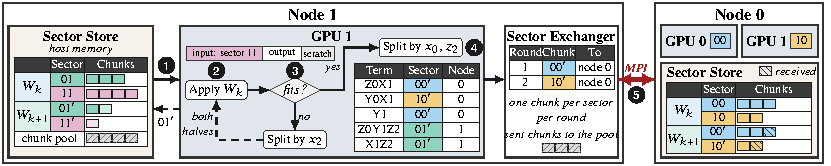
\includegraphics[width=\textwidth]{figures/execution.pdf}
\caption{Host-memory sector execution and boundary exchange with pale filling chunks, black-hatched received chunks, and gray-hatched pooled chunks}
\label{fig:execution}
\end{figure}

\subsection{Implementation}
\SectorQ implements the host runtime in C++ and the string partition operations in CUDA.
Each MPI rank owns one node and creates one worker per GPU, with four GPUs per node in our experiments.

\noindent\textbf{Runtime and Library Operations.}
Each worker uses \cuPP~v0.5.0 on one GPU.
The library operations cover rotations, Clifford gates, Pauli noise, merging, and truncation.
The runtime supplies the sector contents and manages their placement, while the library supplies the arithmetic on each expansion.
CUDA kernels evaluate the row parities and group output terms by their next sectors.
The CPU handles binary elimination, sample scoring, the host chunk pool, and MPI exchange.
Consecutive Pauli noise channels can share a library call up to the next truncation, preserving the scheduled coefficient decisions.
On one GPU, an expansion below the target sector size can remain in device memory between windows.
This path avoids a host transfer when no other worker could receive a sector.
Both optimizations preserve the window partition and its scheduled coefficient decisions.
Table~\ref{tab:parameters} summarizes the default parameters and the larger sector caps used in the capacity experiments.

\begin{table}[t]
\caption{Runtime parameters}
\label{tab:parameters}
\centering
\small
\begin{tabular}{@{}ll@{}}
\toprule
\textbf{Parameter} & \textbf{Setting} \\
\midrule
Sample target across nodes & 200,000 terms \\
Candidate row sets & 8 \\
Target sector input & 4 million terms, 6 million for kicked Ising \\
Tasks per GPU & 1, or 2 after a window of at least 0.5~s \\
Default sector cap & 256 \\
Capacity experiment sector caps & 1,024 or 4,096 \\
Host chunk capacity & 262,144 terms, 65,536 for selected large runs \\
GPU memory budget & 90\% of available device memory \\
Each expansion buffer & 20\% of the GPU memory budget \\
Coefficient truncation & Every 10 operations by default \\
\bottomrule
\end{tabular}
\end{table}

\section{Evaluation}
\label{sec:eval}

\subsection{Evaluation Setup}
We evaluate performance and capacity, the contribution of the design choices, numerical agreement, and sensitivity to execution parameters.

\noindent\textbf{Hardware Specification.}
All experiments use NERSC Perlmutter GPU nodes, each with four NVIDIA A100 GPUs with 40~GB of device memory each, a 64-core CPU, and 256~GiB of host memory.
The nodes communicate over the Slingshot network.
GPU implementations use 90\% of available device memory, approximately 36~GB per GPU.
\SectorQ assigns one MPI rank to each node and one worker to each GPU, whereas distributed \cuPP assigns one rank to each GPU.
The largest configuration contains 128 nodes and 512 GPUs.
CPU implementations use the same nodes as the corresponding GPU configuration.
ORQA uses 64 ranks per node, MonoProp uses eight ranks with eight threads each, and threaded single-node implementations use 64 threads.
Qiskit uses one thread.
The comparisons identify the node count and execution devices rather than assuming equivalent CPU and GPU resources.

\noindent\textbf{Evaluation Scope.}
The experiments measure Heisenberg-picture propagation that returns an observable expectation value.
Unless stated otherwise, each setting is measured once with a 40-minute limit.
The size and exact-reference experiments use a 20-minute limit, and capacity ladders allow \SectorQ up to two hours per run.
A ladder stops after memory exhaustion or its time limit, and an unexecuted point is not a measured failure.
Times cover propagation rather than queue or process-launch delays, including initialization performed lazily within the timed region.
Horizontal-axis term counts denote the largest population at a \SectorQ window boundary under the stated truncation rule.
These counts differ from intermediate expansion within a window and the final output size.
Separate experiments assess numerical error and repeated-run variability.
Thus, the main sweeps compare completed propagations under explicit input, truncation, resource, and timing conditions.

\noindent\textbf{Circuits.}
The seven circuits in Table~\ref{tab:windows} vary the interaction graph, gate family, and observable.
The principal workload is a 127-qubit heavy-hex kicked Ising circuit with 20 steps and rotation angle $\pi/4$.
A second heavy-hex circuit uses transverse-field Ising model (TFIM) rotations at general angles, and a noisy variant adds depolarizing channels with probability 0.005.
The remaining circuits are TFIM on an $11\times11$ lattice, XXZ on an $8\times8$ lattice, a 100-qubit QAOA circuit on a random regular graph, and a 100-qubit hardware-efficient ansatz.
Their respective depths are 10 steps, 6 steps, 4 layers, and 16 layers.
The observables include local magnetization and the edge sum of QAOA.
Additional TFIM grids and kicked Ising depths vary circuit dimensions.
Every comparison within a setting preserves the circuit, observable, and initial state.

\noindent\textbf{Baselines.}
The primary baseline is \cuPP~v0.5.0 with the original circuit and its default distributed mode.
The second baseline uses a Clifford-frame input and defers global deduplication until truncation, with additional merges where required to fit memory.
We report the fastest successful deferred interval among those tested.
The paulistrings-rs comparison uses original gates and truncation after each operation in both systems to match its gate-level coefficient decisions.
Other comparisons use the authors' SPD, MonoProp, PauliPropagation.jl, and ppvm implementations, Qiskit's Pauli propagation package, and our reproduction of ORQA.
These external implementations, except paulistrings-rs, receive the exported Clifford-frame operation list.
MonoProp has a different truncation rule, and its times do not represent equal-error comparisons.
The ORQA results describe our reproduction rather than the authors' implementation.
These distinctions apply throughout the performance comparisons below.

\subsection{Performance Compared with Existing Systems}
We compare implementations from one node to 128 GPUs, retaining separate experiments when their truncation schedules differ.

\noindent\textbf{Single-Node Performance.}
Figure~\ref{fig:single} establishes the arithmetic and capacity behavior before inter-node exchange.
Across circuits that fit one GPU, the ratio of the \cuPP time to the \SectorQ time is 0.6-1.5.
SPD is up to 2.9 times faster on one GPU, but its kicked Ising run exhausts memory at cutoff $10^{-5}$.
At their shared cutoff $3\times10^{-5}$, \SectorQ on four GPUs takes 5.25~s and distributed \cuPP takes 44.3~s.
\SectorQ also completes $3\times10^{-6}$ in 436~s.
At the largest shared settings across circuits, the four-GPU implementation is 108-269 times faster than PauliPropagation.jl, 157-755 than ppvm, and over 1,800 than single-threaded Qiskit.
The ORQA reproduction is 18-71 times slower on the same node.
MonoProp remains faster on several small settings below two seconds, including kicked Ising at $10^{-3}$.
The single-node result therefore includes both the small-problem advantages of other implementations and the broader executable range of \SectorQ.

\begin{figure}[t]
\centering
\panel{ev_single_legend}\\[-2pt]
\panel{ev_single_a}
\caption{Simulation time on one node (4 GPUs)}
\label{fig:single}
\end{figure}

\noindent\textbf{Seven Circuits on 16 GPUs.}
Figure~\ref{fig:circuits} compares the seven circuits on four nodes.
At the largest setting completed by the original-circuit \cuPP baseline for each circuit, \SectorQ is 4.4-9.7 times faster.
Deferred deduplication remains 2.2-4.6 times slower at the shared settings and exhausts memory in two circuits at the primary baseline's largest completed setting.
\SectorQ completes lower cutoffs in all seven circuits, including TFIM and XXZ inputs without removable Clifford gates.
The improvement therefore extends beyond Clifford preprocessing.
The same measurements yield 17-130~ns per boundary term for \SectorQ at settings above 100 million terms, compared with 908-39,000~ns for the primary baseline at cutoff $10^{-4}$.
This normalization divides propagation time by the largest boundary count, rather than measuring one gate application.
It relates the time curves to the operator sizes already shown on their axes, with no assumption of identical work per term across circuits.
% The ev_cost panels normalize these same time measurements by boundary count.
% Their summary is integrated here rather than repeating a seven-panel figure.

\begin{figure}[t]
\centering
\panel{ev_circuits_legend}\\[-2pt]
\subfloat[Kicked Ising]{\panel{ev_circuits_a}}\hfill
\subfloat[TFIM heavy-hex]{\panel{ev_circuits_b}}\hfill
\subfloat[Noisy kicked Ising]{\panel{ev_circuits_c}}\hfill
\subfloat[TFIM $11{\times}11$]{\panel{ev_circuits_d}}\\
\subfloat[XXZ $8{\times}8$]{\panel{ev_circuits_e}}\hfill
\subfloat[QAOA]{\panel{ev_circuits_f}}\hfill
\subfloat[Ansatz]{\panel{ev_circuits_g}}
\caption{Simulation time of seven circuits on 16 GPUs}
\label{fig:circuits}
\end{figure}

\noindent\textbf{Three Circuits on 128 GPUs.}
Figure~\ref{fig:circuits128} extends the comparison to 32 nodes with completed original-circuit \cuPP sweeps.
Kicked Ising and its noisy variant use those original inputs, while the TFIM input is identical with and without a Clifford frame.
At the largest setting completed by the primary baseline in each sweep, \SectorQ is 7.4-13.4 times faster.
For kicked Ising at cutoff $5\times10^{-6}$, the times are about 7.6 and 101.6~s.
The CPU comparisons use the same 32 nodes.
MonoProp remains competitive at the smallest settings, subject to its different truncation rule.
The additional CPU ladders remain incomplete, and their curves end at the last completed point.
This comparison establishes the benefit relative to other systems at a larger resource count, while the scaling experiments below measure the effect of adding resources to \SectorQ itself.
% TBD: append completed CPU ladders from job 59768998.

\begin{figure}[t]
\centering
\panel{ev_circuits128_legend}\\[-2pt]
\subfloat[Kicked Ising]{\panel{ev_circuits128_a}}\hfill
\subfloat[TFIM heavy-hex]{\panel{ev_circuits128_b}}\hfill
\subfloat[Noisy kicked Ising]{\panel{ev_circuits128_c}}
\caption{Three circuits on 128 GPUs with original-circuit primary baselines}
\label{fig:circuits128}
\end{figure}

\noindent\textbf{Fixed-Partition Implementation with Matched Truncation.}
Figure~\ref{fig:prs} compares \SectorQ with paulistrings-rs on 16 GPUs using truncation after each operation and the same original circuit.
The fixed partition uses the library's seeded rows.
\SectorQ is 1.6-5.4 times faster over all 30 shared settings and 1.6-4.1 times faster at the largest shared setting of each circuit.
At the next tested cutoff in five circuits, paulistrings-rs exhausts GPU memory while \SectorQ completes in 29-880~s.
Small-setting times include any lazy GPU kernel compilation in the propagation call.
These curves remain separate from Figure~\ref{fig:circuits} because its default truncation interval differs.
The comparison measures complete implementations, including their arithmetic and storage choices.
Section~\ref{sec:design-eval} isolates row recomputation within the same engine, and Section~\ref{sec:accuracy} reports numerical agreement for the matched schedules.
% TBD: paulistrings-rs 32/64 GPU results from jobs 59769001 and 59769002.

\begin{figure}[t]
\centering
\panel{ev_prs_legend}\\[-2pt]
\subfloat[Kicked Ising]{\panel{ev_prs_a}}\hfill
\subfloat[TFIM heavy-hex]{\panel{ev_prs_b}}\hfill
\subfloat[Noisy kicked Ising]{\panel{ev_prs_c}}\hfill
\subfloat[TFIM $11{\times}11$]{\panel{ev_prs_d}}\\
\subfloat[XXZ $8{\times}8$]{\panel{ev_prs_e}}\hfill
\subfloat[QAOA]{\panel{ev_prs_f}}\hfill
\subfloat[Ansatz]{\panel{ev_prs_g}}
\caption{\SectorQ and fixed linear partitions on 16 GPUs}
\label{fig:prs}
\end{figure}

\subsection{Scalability and Capacity}
We vary the GPU count, circuit dimensions, and retained operator size to distinguish execution scaling from capacity.

\noindent\textbf{Strong Scalability.}
For fixed large problems, \SectorQ achieves speedups of 81-166 on 256 GPUs and 83-180 on 512 GPUs relative to one GPU.
The representative settings are kicked Ising at cutoff $3\times10^{-6}$ and heavy-hex TFIM and noisy kicked Ising at $5\times10^{-6}$.
Figure~\ref{fig:scaleout} also shows the kicked Ising cutoff ladder from one to 512 GPUs.
The gain beyond 256 GPUs is modest under the default cap of 256 sectors.
At kicked Ising cutoff $3\times10^{-6}$, time decreases from 10.48 to 9.67~s.
The trace has at most 256 nonempty sectors and no GPU splits, limiting concurrent sector execution below the 512 workers.
Small problems also saturate, with cutoff $10^{-5}$ near three seconds from 128 GPUs onward.
The time decomposition in Section~\ref{sec:design-eval} relates this limit to worker idle time and the remaining fixed costs.

\begin{figure}[t]
\centering
\panel{ev_scaleout_legend}\\[-2pt]
\panel{ev_scaleout_a}
\caption{Kicked Ising propagation from 1 to 512 GPUs}
\label{fig:scaleout}
\end{figure}

\noindent\textbf{Weak Scalability.}
Figure~\ref{fig:weak} increases the boundary term count with the GPU count by lowering the cutoff.
Efficiency is boundary-term throughput per GPU relative to the corresponding one-GPU run, accounting for the counts actually produced.
For the large load, \SectorQ retains 80-88\% of this throughput on 16 GPUs and 72-80\% on 64 GPUs across the three circuits.
The range falls to 23-38\% on 512 GPUs under the default sector cap.
The measured \cuPP large-load configurations exhaust GPU memory, whereas the small load permits time comparisons on both systems.
On 16 GPUs, \SectorQ is 8.1-12 times faster than the original-circuit baseline for the small load.
CPU results appear where completed, with missing measurements omitted rather than interpreted as failures.
Together, the weak and strong sweeps show that capacity continues to grow after the throughput per GPU decreases.
% TBD: remaining CPU and 512-GPU baseline weak points from the fill campaign.

\begin{figure}[t]
\centering
\panel{ev_weak_legend}\\[-2pt]
\subfloat[Kicked Ising, small load]{\panel{ev_weak_a}}\hfill
\subfloat[TFIM heavy-hex, small load]{\panel{ev_weak_b}}\hfill
\subfloat[Noisy kicked Ising, small load]{\panel{ev_weak_c}}\\
\subfloat[Kicked Ising, large load]{\panel{ev_weak_d}}\hfill
\subfloat[TFIM heavy-hex, large load]{\panel{ev_weak_e}}\hfill
\subfloat[Noisy kicked Ising, large load]{\panel{ev_weak_f}}
\caption{Weak scaling from 1 to 512 GPUs}
\label{fig:weak}
\end{figure}

\noindent\textbf{Circuit Size and Depth.}
Figure~\ref{fig:size} varies the TFIM lattice size and kicked Ising depth on 16 GPUs.
The lattice sweep covers 36-1,024 qubits with total magnetization as the observable, changing string length, graph size, and observable size together.
At 1,024 qubits on a $32\times32$ lattice, \SectorQ completes in 90.4~s and is 4.1 times faster than original-circuit \cuPP.
This qubit count is the supported library limit in the experiment, not a measured limit of the partition rule.
The depth sweep keeps the kicked Ising graph fixed and increases its Trotter steps.
At 60 steps, \SectorQ takes 160~s and is 50 times faster than the primary baseline.
Longer propagation changes both the number of windows and the surviving operator, without implying proportional growth in retained terms.
These two sweeps extend the result beyond the main circuit dimensions without extrapolating cost from qubit or gate count alone.

\begin{figure}[t]
\centering
\panel{ev_size_legend}\\[-2pt]
\subfloat[Qubits, cutoff $10^{-3}$]{\panel{ev_size_a}}\hfill
\subfloat[Qubits, cutoff $10^{-4}$]{\panel{ev_size_b}}\hfill
\subfloat[Trotter steps]{\panel{ev_size_c}}
\caption{Simulation time by circuit size and depth}
\label{fig:size}
\end{figure}

\noindent\textbf{Largest Operator and Host Memory.}
The capacity ladder reaches 448.2 billion boundary terms on 512 GPUs at cutoff $1.5\times10^{-7}$, completing in 3,413~s.
The 17.9~TB expansion is 140 times larger than the largest completed original-circuit \cuPP setting on the same GPUs, 3.2 billion terms at $2\times10^{-6}$.
The host chunk pool occupies 21,079~GiB across 128 nodes, 64\% of installed host memory.
This allocation includes reusable chunks and transient storage, rather than measuring the processes' total resident memory.
Round-based exchange limits additional receive storage, and each sector must still admit a finer valid partition if its working set exceeds GPU memory.
On 128 GPUs, \SectorQ completes 117.5 billion terms.
The 256-GPU endpoint remains under remeasurement after a stalled run.
We distinguish completed runs, measured failures, and settings rejected from estimated storage requirements.
The 140-fold comparison is specifically against \cuPP and does not establish a capacity advantage over every CPU implementation.
% TBD: 256-GPU endpoint and CPU reach from jobs 59768854 and the fill campaign.

\subsection{Contribution of the Design Choices}
\label{sec:design-eval}
We combine controlled changes to the engine with time counters to identify the source and limits of the observed gains.

\noindent\textbf{Preprocessing and Window Sectors.}
Figure~\ref{fig:staircase} measures successive changes on kicked Ising at cutoff $10^{-5}$ and 16 GPUs.
The original-circuit \cuPP baseline takes 95.0~s.
A Clifford-frame input reduces time to 54.3~s, and deferred global deduplication reduces it to 48.8~s.
Window-sector execution reaches 12.2~s with the same underlying library operations.
This sequence separates the benefit of preprocessing from the execution structure built around those operations.
It also shows that fewer global merges alone do not account for the observed time reduction.
The fixed-row experiment below further tests whether one partition chosen in advance can obtain the same effect.
Its recomputed run takes 11.9~s at this setting, from a separate allocation.
We retain the two measurements separately rather than treating their small difference as the effect of another design change.
Together, the experiments distinguish the execution mechanism from implementation differences between simulators.

\begin{figure}[t]
\centering
\panel{ev_staircase_legend}\\[-2pt]
\panel{ev_staircase_a}
\caption{Run time as each element is added on 16 GPUs}
\label{fig:staircase}
\end{figure}

\noindent\textbf{Fixed versus Recomputed Rows.}
Figure~\ref{fig:fixedrows} isolates row recomputation with the same Clifford frame, GPU operations, and truncation schedule.
The fixed variant selects rows at the first partitioned window and retains them, ending a window when a rotation changes those rows.
The recomputed variant selects rows for each window.
Fixed rows are 2.4-17.0 times slower over 25 successful pairs on 16 GPUs and 1.3-14.8 times slower over 22 pairs on four GPUs.
All pairs have identical printed expectation values.
Several fixed-row runs exhaust host memory at lower cutoffs that the recomputed variant completes.
Noisy kicked Ising is excluded because the fixed variant does not support its explicit Clifford operations between rotations.
Table~\ref{tab:fixedrows} connects the time difference to window count and traffic.
For kicked Ising at $10^{-5}$, recomputation reduces 878 windows to 20 and 698.5~GB to 45.2~GB, supporting the benefit of window-dependent partitions within one engine.

\begin{figure}[t]
\centering
\panel{ev_fixed_rows_legend}\\[-2pt]
\subfloat[Kicked Ising]{\panel{ev_fixed_rows_a}}\hfill
\subfloat[TFIM heavy-hex]{\panel{ev_fixed_rows_b}}\hfill
\subfloat[TFIM $11\times11$]{\panel{ev_fixed_rows_c}}\\
\subfloat[XXZ $8\times8$]{\panel{ev_fixed_rows_d}}\hfill
\subfloat[QAOA]{\panel{ev_fixed_rows_e}}\hfill
\subfloat[Ansatz]{\panel{ev_fixed_rows_f}}
\caption{Fixed and recomputed rows on 16 GPUs, with fixed-to-recomputed time ratios}
\label{fig:fixedrows}
\end{figure}

\begin{table}[t]
\caption{Windows and inter-node traffic at cutoff $10^{-5}$ on 16 GPUs}
\label{tab:fixedrows}
\centering\small
\begin{tabular}{@{}lrrrr@{}}
\toprule
& \multicolumn{2}{c}{\textbf{Windows}} & \multicolumn{2}{c}{\textbf{Traffic (GB)}} \\
\textbf{Circuit} & \textbf{Recomputed} & \textbf{Fixed} & \textbf{Recomputed} & \textbf{Fixed} \\
\midrule
Kicked Ising & 20 & 878 & 45.2 & 698.5 \\
TFIM heavy-hex & 45 & 2,241 & 79.0 & 342.2 \\
TFIM $11\times11$ & 24 & 1,518 & 60.0 & 625.9 \\
XXZ $8\times8$ & 23 & 1,155 & 44.8 & 2,369.9 \\
QAOA & 8 & 198 & 8.2 & 34.0 \\
Ansatz & 34 & 1,392 & 8.3 & 107.7 \\
\bottomrule
\end{tabular}
\end{table}

% TBD N2: compare candidates 1 and 8 using jobs/b_ablate.sh, logs/b/.
% The 2026-10-15 interactive submission was rejected by QOSMaxSubmitJobPerUserLimit.
% Add Balanced Row Selection here when time, occupancy, split, and answer data exist.
% Distinguish imbalance over nonempty sectors from imbalance over all 2**rows labels.

\noindent\textbf{Time Breakdown across Scales.}
Figure~\ref{fig:runtime} retains cutoff $10^{-4}$ as a small reference and increases the other workloads with the GPU count.
Within each circuit, the middle points keep boundary terms per GPU within a factor of 1.5.
The 64- and 256-GPU capacity points use sector caps of 1,024 and 4,096, with 65,536-term chunks on 256 GPUs.
These profiles assess activity at larger problem sizes, rather than speedup for a fixed input.
Worker counters are divided by the GPU count and compared with wall time.
Library-call time is not sampled GPU utilization.
On 64 GPUs, kicked Ising reaches 44.3 billion boundary terms at the largest point, with 0.7\% average worker idle time.
Five capacity points remain pending, including kicked Ising on 256 GPUs and TFIM and noisy kicked Ising on both larger allocations.

The small reference spends 37-52\% of wall time in average worker idle time across the nine profiles.
At the largest 16-GPU settings, library operations account for 70-89\% and inter-node exchange for 3-13\%.
The original-circuit \cuPP baseline separately records 39-44\% of its large-setting time inside MPI calls.
The separate 512-GPU measurements show that average worker idle time rises from 9\% to 40\% of wall time relative to 256 GPUs at kicked Ising cutoff $3\times10^{-6}$.
The largest capacity run uses a higher sector cap and has a different composition, with 46\% in library calls, 26\% in exchange, and 9\% in GPU-host copies.
Its exchange includes 607~s in transfer, 280~s in posting, and under two seconds in counts.
These measurements distinguish insufficient task concurrency from exchange overhead.

\begin{figure}[tp]
\centering
\panel{ev_runtime_legend}\\[-2pt]
\subfloat[Kicked Ising, 16 GPUs]{\panel{ev_runtime_a}}\hfill
\subfloat[TFIM heavy-hex, 16 GPUs]{\panel{ev_runtime_b}}\hfill
\subfloat[Noisy kicked Ising, 16 GPUs]{\panel{ev_runtime_c}}\\[4pt]
\subfloat[Kicked Ising, 64 GPUs]{\panel{ev_runtime_d}}\hfill
\subfloat[TFIM heavy-hex, 64 GPUs]{\panel{ev_runtime_e}}\hfill
\subfloat[Noisy kicked Ising, 64 GPUs]{\panel{ev_runtime_f}}\\[4pt]
\subfloat[Kicked Ising, 256 GPUs]{\panel{ev_runtime_g}}\hfill
\subfloat[TFIM heavy-hex, 256 GPUs]{\panel{ev_runtime_h}}\hfill
\subfloat[Noisy kicked Ising, 256 GPUs]{\panel{ev_runtime_i}}
\caption{Time shares for a fixed small reference and larger workloads at each GPU count. Parentheses show boundary term counts. Asterisks mark capacity settings with higher sector caps. Pending points have no completed measurement}
\label{fig:runtime}
\end{figure}

\subsection{Numerical Agreement and Accuracy}
\label{sec:accuracy}
Numerical validation separates faithful distributed execution from the approximation introduced by coefficient truncation.

\noindent\textbf{Agreement across Implementations.}
Across 68 circuit-cutoff settings with at least two successful runs under a common truncation rule, the largest absolute expectation difference is $4.9\times10^{-11}$.
This comparison includes the single-GPU reference, distributed \cuPP, and external implementations with the same coefficient decisions.
The largest difference occurs for QAOA's edge-sum observable.
The separate gate-level truncation comparison with paulistrings-rs agrees within $4.7\times10^{-11}$ over 75 completed settings on one, four, and 16 GPUs.
\SectorQ also preserves the printed answer when sector count, GPU count, window rule, or device-memory budget changes.
These checks exercise the partition, exchange, and merge operations across the evaluated configurations.
They validate the distributed implementation of a specified truncation schedule, without establishing that the chosen cutoff approximates the exact quantum expectation sufficiently well.
The exact-reference experiment below tests this separate approximation question.

\noindent\textbf{Error against an Exact Reference.}
Figure~\ref{fig:accuracy} uses a 30-qubit TFIM on a $5\times6$ lattice with an exact state-vector reference, checked against untruncated Pauli propagation on smaller grids.
The four-step circuit reaches absolute error $7.2\times10^{-5}$ at cutoff $10^{-7}$, with \SectorQ on 16 GPUs completing in 29.2~s.
Implementations with the same truncation rule have the same error at a given cutoff, whereas MonoProp requires a separate error comparison.
The six-step circuit reaches time or memory limits at higher cutoffs.
Neither sweep has strictly monotonic error at every intermediate cutoff.
The large kicked Ising workload has no exact reference at the evaluated scale and is also nonmonotonic.
Its values from cutoff $10^{-6}$ to $1.5\times10^{-7}$ are approximately 0.3217, 0.3256, 0.3265, 0.3226, 0.3153, and 0.3089.
Thus, the capacity result extends the accessible truncated computation without asserting convergence or a guaranteed reduction in physical error.

\begin{figure}[t]
\centering
\panel{ev_accuracy_legend}\\[-2pt]
\subfloat[4 Trotter steps]{\panel{ev_accuracy_a}}\hfill
\subfloat[6 Trotter steps]{\panel{ev_accuracy_b}}
\caption{Simulation time and error of a 30-qubit TFIM}
\label{fig:accuracy}
\end{figure}

\subsection{Parameter Sensitivity and Repeatability}
Figure~\ref{fig:robustness} groups parameter changes and repeated measurements to test the stability of the execution behavior.

\noindent\textbf{Sector Granularity and Device Memory.}
At cutoff $10^{-5}$, a target sector size one quarter of the default increases time by 9-26\%, whereas twice the target reduces it by 2-9\% across the representative circuits.
One to four tasks per GPU differ by at most 9\%, and eight can increase time by up to 35\% on 16 GPUs.
The tradeoff is between additional library invocations with small sectors and working-buffer pressure with large sectors.
Reducing the device-memory budget from 36 to 4~GB increases time by 12-64\% but preserves the tested answers through finer sector execution.
More concurrency alone is not sufficient at large scale.
A 512-GPU kicked Ising run at $3\times10^{-6}$ with a 4,096-sector cap and smaller host chunks takes 11.6~s, against the default's 9.7~s.
This joint change does not isolate the cap and does not establish one configuration as optimal across cluster sizes.

\noindent\textbf{Repeated Measurements.}
The repetition experiment contains 160 completed kicked Ising runs, with ten measurements per setting.
We define spread as maximum minus minimum time divided by their mean.
On 16 GPUs, spread is 1.4-7.2\% for \SectorQ and 3.4-7.6\% for original-circuit \cuPP.
All repetitions preserve the printed expectation value.
Each system's 16-GPU repetitions use one allocation, but the systems use different allocations.
This avoids allocation changes within a system's spread while retaining that distinction in the comparison.
At cutoff $10^{-5}$, the ratio of ten-run means is 7.6, close to the main sweep's single-run ratio of 7.8.
Panels (d) and (e) show the repeated times across problem sizes and GPU counts, respectively.
The repetition results support the observed performance difference without treating a single-run measurement as a confidence interval.

\begin{figure}[tp]
\centering
\panel{ev_knobs_legend}\\[-2pt]
\subfloat[Target terms per sector]{\panel{ev_knobs_a}}\hfill
\subfloat[Sectors per GPU]{\panel{ev_knobs_b}}\hfill
\subfloat[GPU memory allowed]{\panel{ev_knobs_c}}\\[4pt]
\panel{ev_variability_legend}\\[-2pt]
\subfloat[Repetitions on 16 GPUs by problem size]{\panel{ev_variability_a}}\hfill
\subfloat[Repetitions at cutoff $3{\times}10^{-5}$ by GPU count]{\panel{ev_variability_b}}
\caption{Parameter sensitivity at cutoff $10^{-5}$ and ten repeated measurements of kicked Ising}
\label{fig:robustness}
\end{figure}

\section{Related Work}
\label{sec:related}
The relevant distinctions concern the partition rule, when it changes, and the memory that holds the propagated operator.

\noindent\textbf{Conserved Operator Subspaces.}
Symmetries and invariant subspaces are established tools in quantum simulation.
Bravyi et al. identify binary symmetries of fermionic Hamiltonians and remove qubits after selecting a symmetry sector~\cite{bravyi2017tapering}.
West et al. describe a commutator graph whose connected components identify invariant operator subspaces under a set of generators~\cite{west2025graph}.
These results establish the algebraic basis for independent evolution and preclude a novelty claim based on parity conservation alone.
\SectorQ uses binary rows as labels on Pauli strings, with the ordinary binary inner product expressing invariance under generator XOR.
The labels are not symmetry eigenvalues of a quantum state, and their sectors need not be individual connected components of the commutator graph.
The system derives sufficiently fine labels for a finite window and replaces them when the next window has different generators.
This construction supplies an executable partition for distributed merge and truncation without requiring a useful nontrivial partition conserved by the entire circuit.

\noindent\textbf{Fixed Linear Partitions.}
The closest implementation-level comparison is paulistrings-rs, whose partition label is a binary matrix times the Pauli bit vector~\cite{paulistrings}.
Its linear map identifies one communication partner for each nonlocal generator delta, and its local coset execution already exploits independent groups of strings.
The documented partition rows remain fixed during a run, and automatic row selection that accounts for both balance and remote work is listed as an open problem.
The parallel iQCC implementation also uses a bitmask to assign Pauli words to processes and computes the destination of a product through XOR~\cite{genin2025chemistry}.
A predictable destination can still be remote.
\SectorQ requires every chosen row to annihilate every generator in the current window, placing all resulting merge partners in one sector throughout that window.
It then selects rows again for the next window and schedules sectors from host memory.
Our same-engine fixed-row ablation isolates this temporal choice, while the paulistrings-rs comparison measures complete implementations with matched truncation.

\noindent\textbf{Distributed CPU Propagation.}
ORQA demonstrates large-scale propagation on Fugaku with up to one trillion Pauli strings and $2^{17}$ processes~\cite{orqa}.
Its distribution map is a structured enumeration of string bits designed to limit communication partners while maintaining balance.
It is not a generic hash, and the sparsity of its communication is central to its scaling.
The map still distributes updates as the propagation advances through generators, rather than deriving a partition conserved by a window.
MonoProp provides distributed Pauli and Majorana propagation through a C++ implementation with Python interfaces~\cite{monoprop}.
These systems establish that large operators can reside in distributed CPU memory.
\SectorQ addresses the additional requirement of executing sectors through GPU kernels while the operator remains in host memory.
Our evaluation labels the ORQA implementation as a reproduction, identifies the CPU resources used, and treats MonoProp's different truncation rule separately from comparisons with identical coefficient decisions.

\noindent\textbf{Propagation Libraries and GPU Kernels.}
Sparse Pauli dynamics and PauliPropagation.jl develop efficient observable simulation and truncation methods~\cite{begusic2024fast,rudolph2025pauli}.
Quantinuum's SPD provides GPU execution, and Qiskit's Pauli propagation package supports Clifford operations, Pauli rotations, and noise channels~\cite{spd,qiskitpauliprop}.
These libraries improve the cost and coverage of propagation within their supported execution environments.
NVIDIA's \cuPP supplies GPU operations on sparse Pauli expansions and a distributed execution mode~\cite{cupauliprop}.
\SectorQ uses its single-GPU operations for arithmetic and compares against its original-circuit distributed mode.
Consequently, the contribution concerns the locality and storage of those operations, not a replacement arithmetic kernel.
The measured element sequence separates Clifford preprocessing and deferred deduplication from window-sector execution.
The single-GPU comparison also retains cases in which another implementation is faster.
This distinction identifies the system benefit as the ability to execute growing operators across nodes without requiring the complete local expansion to remain in GPU memory.

\noindent\textbf{Repeated Evaluations and Gradients.}
PADO-Pauli compiles circuits and observables into sparse matrices that are reused for batches of parameter values and supports gradients through PyTorch~\cite{kim2026pado}.
Its reuse of a compiled representation targets repeated evaluations during variational training.
Backpropagating Pauli Propagation develops gradient evaluation whose computational complexity matches forward propagation and reduces its memory requirements through reversibility~\cite{lin2026backpropagating}.
These objectives differ from the single forward propagation measured in our capacity and scaling experiments.
\SectorQ follows the surviving terms of one specified circuit and cutoff, with new rows chosen from those live terms at window boundaries.
It neither assumes a fixed sparse program shared by parameter batches nor evaluates derivatives in the reported experiments.
The distinction is relevant because a faster batched or gradient evaluation is not directly comparable to the time of a single forward run with the same coefficient truncation.
The methods address complementary workloads, and their integration would require a separate numerical and performance evaluation.

\noindent\textbf{Staged State Vector Simulation.}
State vector simulators already reduce communication through groups of gates.
H\"aner and Steiger schedule gates to reduce communication in a distributed simulation of 45 qubits~\cite{haner2017petabyte}.
Atlas partitions circuits into stages with an integer program, selects kernels with dynamic programming, and supports host-memory offloading~\cite{xu2024atlas}.
Stage boundaries and host storage are therefore not new independently.
Their state vector has a fixed index space, whereas Pauli propagation creates strings, combines equal strings, and removes coefficients during execution.
A useful partition must preserve these merges before truncation, and the sizes of its parts depend on the surviving operator.
\SectorQ derives this locality from the window generators and obtains execution granularity from a sample of the live terms.
An oversized sector can be subdivided only by rows valid for its remaining operations.
This constraint connects host-memory execution to the algebraic partition and distinguishes the proposed mechanism from applying a state-vector stage schedule to a sparse operator.

\section{Conclusion}
\label{sec:conclusion}
% FORMAT: three sentences, 85-120 words, no future work. DRAFT (2026-10-14)
In this paper, we design and implement \SectorQ, a Pauli propagation system for GPU clusters that partitions the terms by the parities that each window of gates conserves.
By recomputing these parities for every window from the generators of its gates and the live terms, we confine the merging of terms to one sector during a window and hold the sectors in host memory.
We evaluate \SectorQ with seven circuits on up to 512 NVIDIA A100 GPUs, reducing the simulation time of \cuPP by 4.4-9.7$\times$ on 16 GPUs and increasing the largest finished problem by 140$\times$ on 512 GPUs through exchanges at window boundaries and sectors in host memory.


\bibliographystyle{ACM-Reference-Format}
\bibliography{paper}

\end{document}
